The interface of our System is to be used via a mobile app because all the functionality make sense only in a \textit{movable} context (meaning that users can exploit them anywhere they have an internet connection).

We will now list some of the user interfaces thought for \textit{Travlendar+}:

% login %
\begin{figure}[h]
	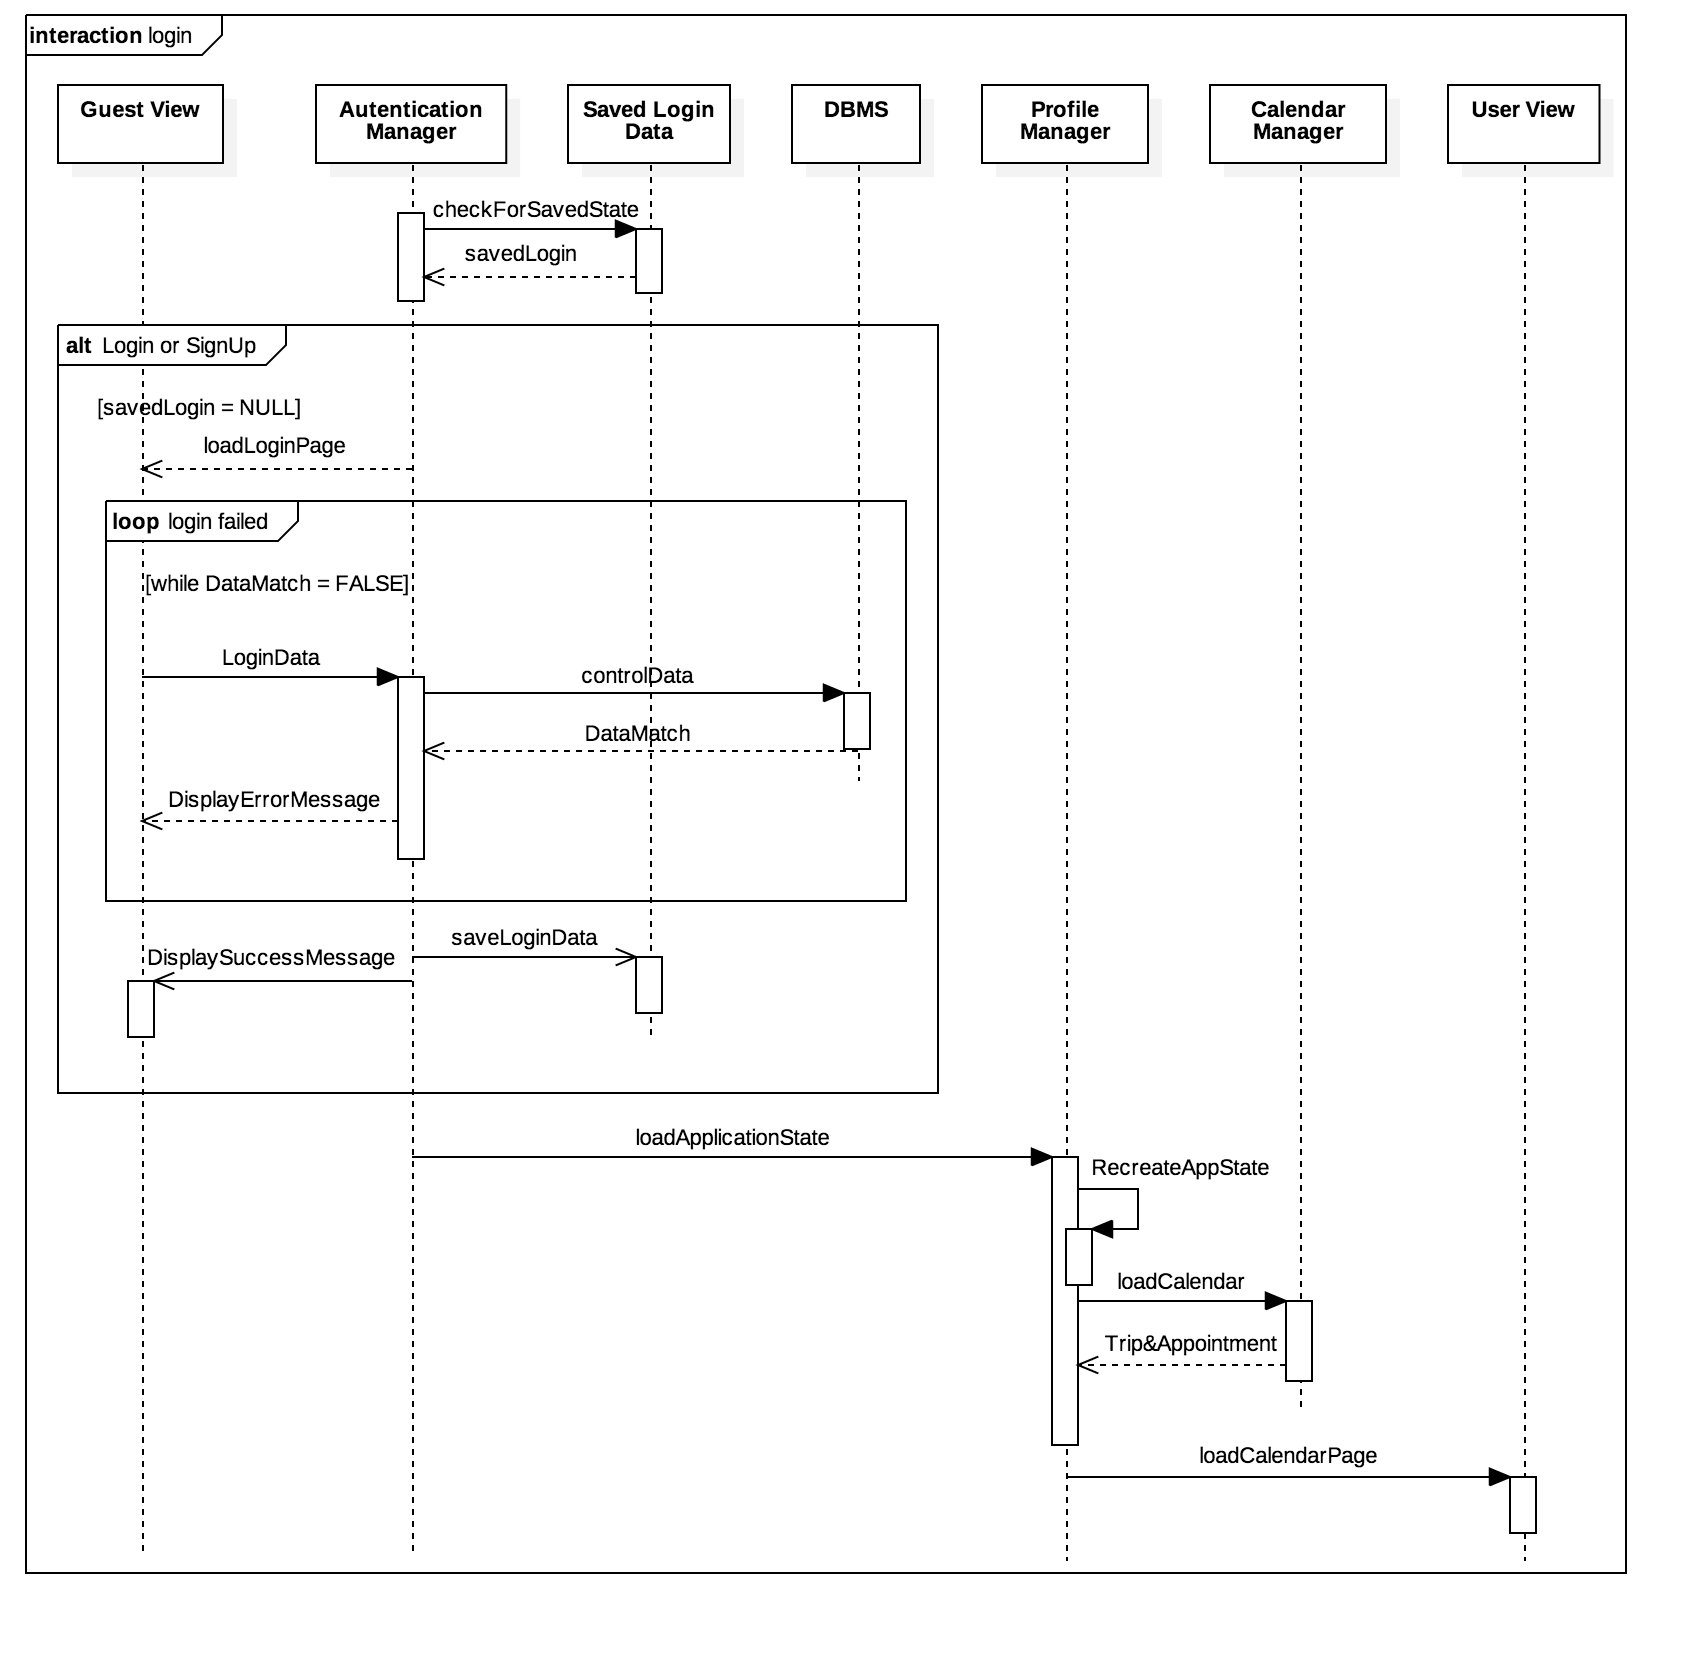
\includegraphics[width=4cm, height=8.5cm]{mockup/login}
	\centering
	\caption{Login Page.}
	\label{fig:login}
\end{figure}
	As mentioned before, a \textit{Guest} or a \textit{non logged User} will first encounter the page showed in figure \ref{fig:login}, and he won't be able to access the app until he completes the Registration or the Login procedures (see sections \ref{register_useCase} and \ref{login_useCase}).


% home page %

\begin{figure}[H]
	\begin{subfigure}{0.5\textwidth}
		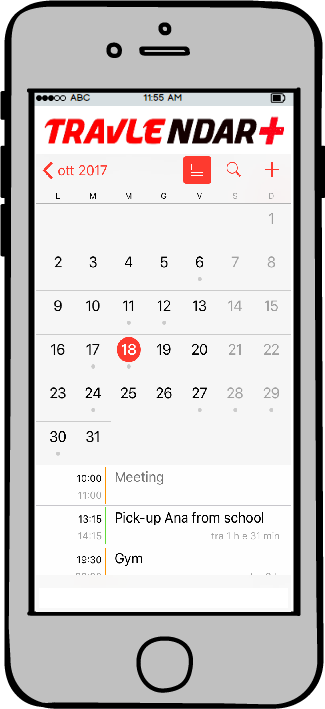
\includegraphics[width=4cm, height=8.5cm]{mockup/homepageMonth} 
		\centering
		\caption{Home Page in Monthly view.}
		\label{fig:homePage_Month}
	\end{subfigure}
	\begin{subfigure}{0.5\textwidth}
		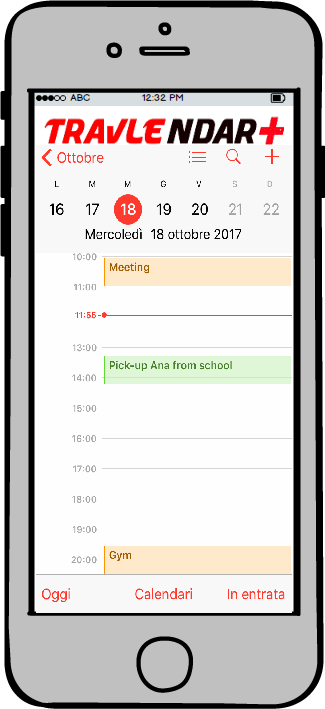
\includegraphics[width=4cm, height=8.5cm]{mockup/homepageDaily} 
		\centering
		\caption{Home Page in Daily view.}
		\label{fig:homePage_Day}
	\end{subfigure}
	\caption{Samples of view events.}
\end{figure}

	The user can use two different views to manage events in his homepage. On the left (figure \ref{fig:homePage_Month}) the application shows monthly view, on the right (figure \ref{fig:homePage_Day}) the daily view. Thus user will modify the scheduling in a simple way by clicking on the events.


% create Event %

\begin{figure}[H]
	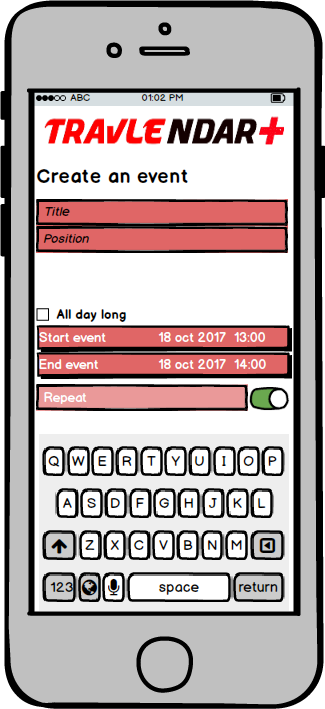
\includegraphics[width=4cm, height=8.5cm]{mockup/createAnEvent}
	\centering
	\caption{Create an Appointment page.}
	\label{fig:createEvent}
\end{figure}
	
	When the user wants to creates an event, he has to use this interface of the application. In fact figure \ref{fig:createEvent} shows what preferences the user can choose regarding the event.


% travel Logic %

\begin{figure}[H]	
	\begin{subfigure}{0.5\linewidth}
		\centering		
		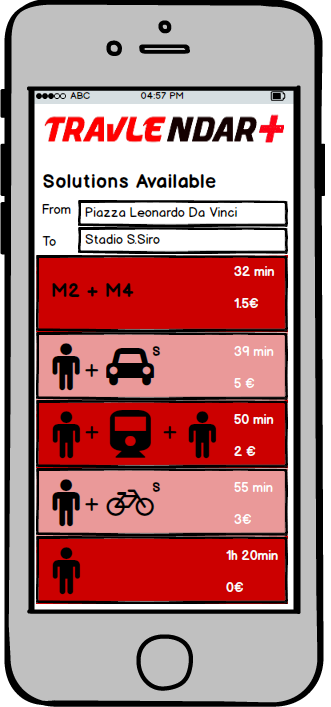
\includegraphics[width=4cm, height=8.5cm]{mockup/solutions} 
		\caption{Solutions found for an Event view.}
		\label{fig:solutions}
	\end{subfigure}
	\begin{subfigure}{0.5\linewidth}
		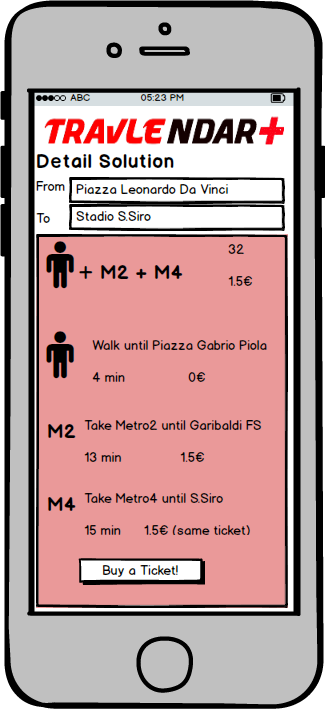
\includegraphics[width=4cm, height=8.5cm]{mockup/buyATicket} 
		\centering
		\caption{Buy a public transportation ticket view.}
		\label{fig:buyTicket}
	\end{subfigure} 
	\hfill
	
	\bigskip	
	\begin{subfigure}{\linewidth}
			\centering
		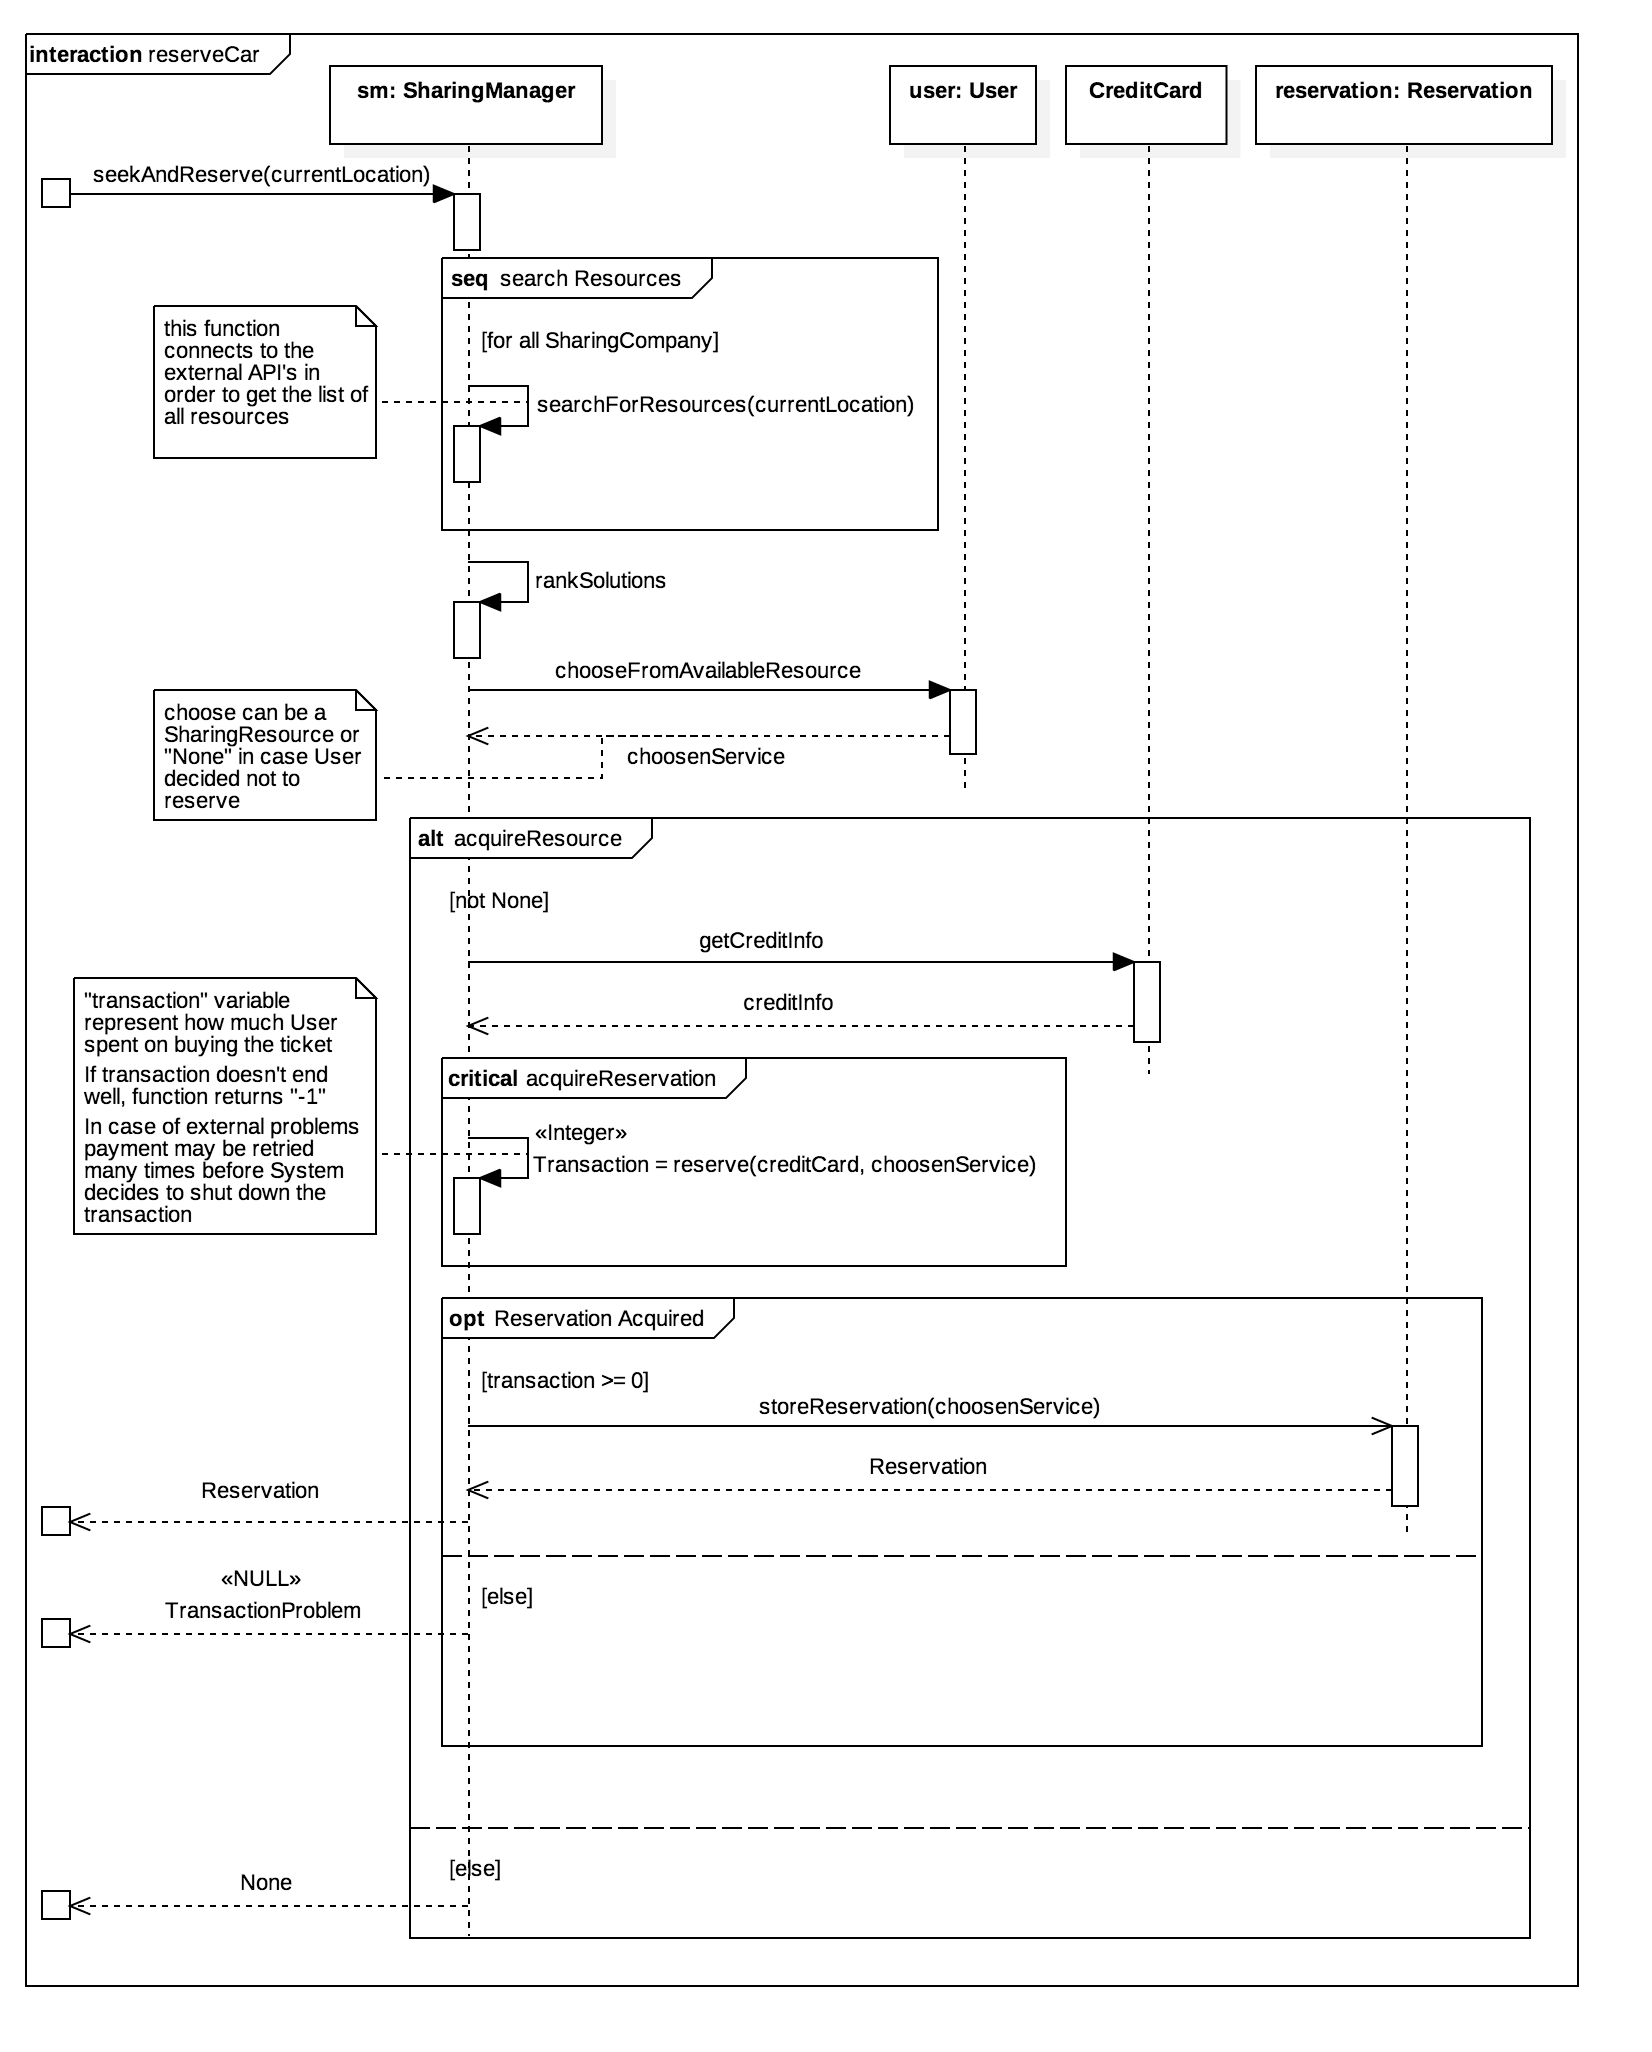
\includegraphics[width=4cm, height=8.5cm]{mockup/reserveCar} 
		\caption{Reserve a Sharing service resource view.}
		\label{fig:reserveCar}
	\end{subfigure}

	\caption{Samples of the Travel logic module.}
	\label{fig:travelLogic}
\end{figure}

	The application computes the possible solutions to reach a certain event based on the starting position. These are displayed on the screen of the user's smartphone as shown in figure \ref{fig:solutions}. The user must choose the preferred solution to see the details. It may happen that the solution contains 'buy tickets' (figure \ref{fig:buyTicket}) or 'hire cars' (figure \ref{fig:reserveCar}). Clicking on the corresponding buttons will open the corresponding externarl application.
